\documentclass{article}
\usepackage{graphicx}
\usepackage{subcaption}

\title{Weekly meeting notes}
\author{Eugenio Pescimoro }

\begin{document}

\maketitle

\section{Introduction}
The aim of these notes is to describe one of the available numerical methods for modelling the diffusion and reaction processes of liquid chemical compounds displacing through fractured porous media.

\begin{figure}[htbp]
    \centering
    \begin{subfigure}[b]{0.45\textwidth}
        \centering
        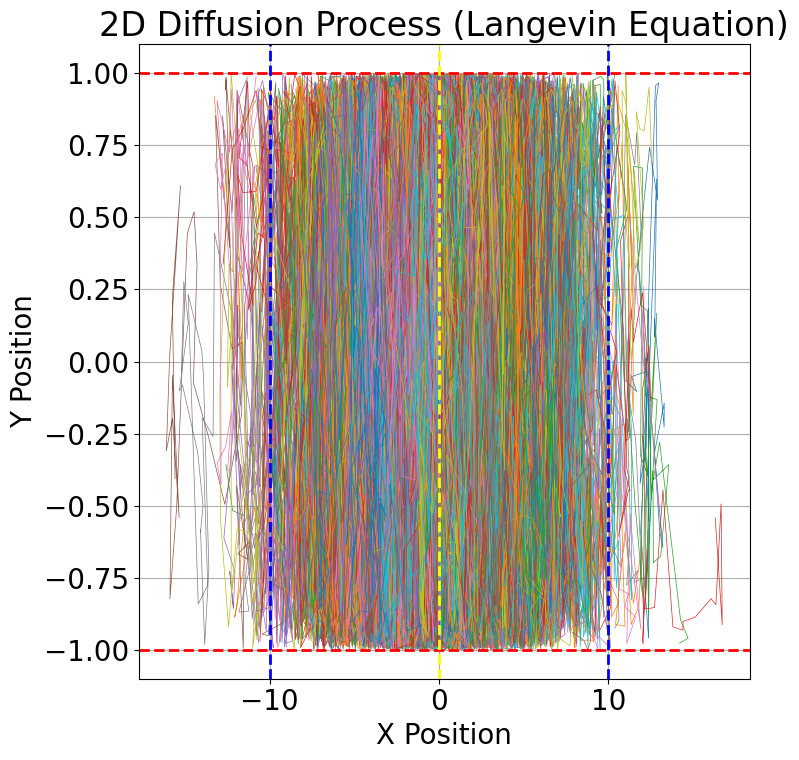
\includegraphics[width=\textwidth]{images/trajectoriesInfinite.png} % Replace with your image path
        \caption{Trajectories of 1e4 particles during 1e3 time steps}
        \label{fig:subplotTrInf}
    \end{subfigure}
    \hfill
    \begin{subfigure}[b]{0.45\textwidth}
        \centering
        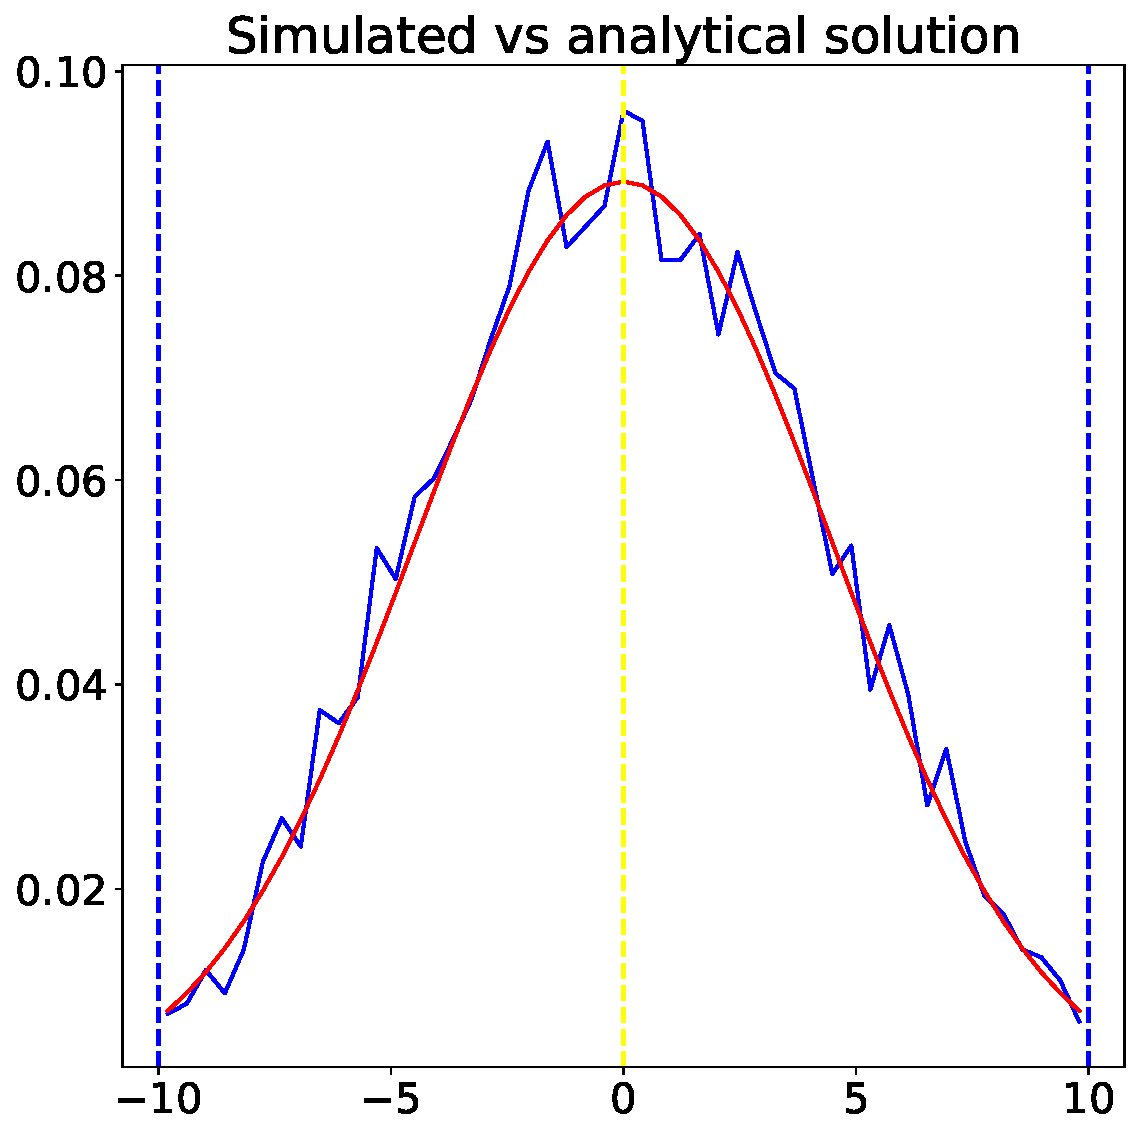
\includegraphics[width=\textwidth]{images/verificationInfinite.pdf} % Replace with your image path
        \caption{Spatial distribution of the particles at time 1e2}
        \label{fig:subplotVerInf}
    \end{subfigure}
    \caption{Verification of the code comparing two spatial distribution of the concentration at a given time: solid blue line represents the spatial concentration from a numerical simulation while solid red line shows the analytical solution of the spatial concentration in a infinite domain at the same given time}
    \label{fig:Infinite}
\end{figure}

\begin{figure}[htbp]
    \centering
    \begin{subfigure}[b]{0.45\textwidth}
        \centering
        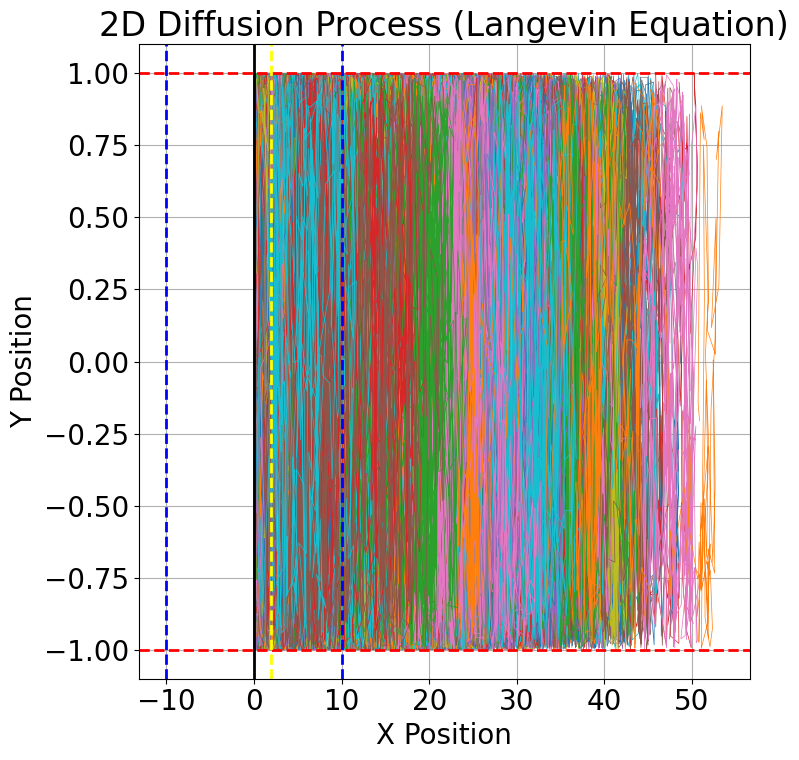
\includegraphics[width=\textwidth]{images/trajectoriesSemiInfinite.png} % Replace with your image path
        \caption{Trajectories of 1e4 particles during 1e3 time steps}
        \label{fig:subplotTrSemiInf}
    \end{subfigure}
    \hfill
    \begin{subfigure}[b]{0.45\textwidth}
        \centering
        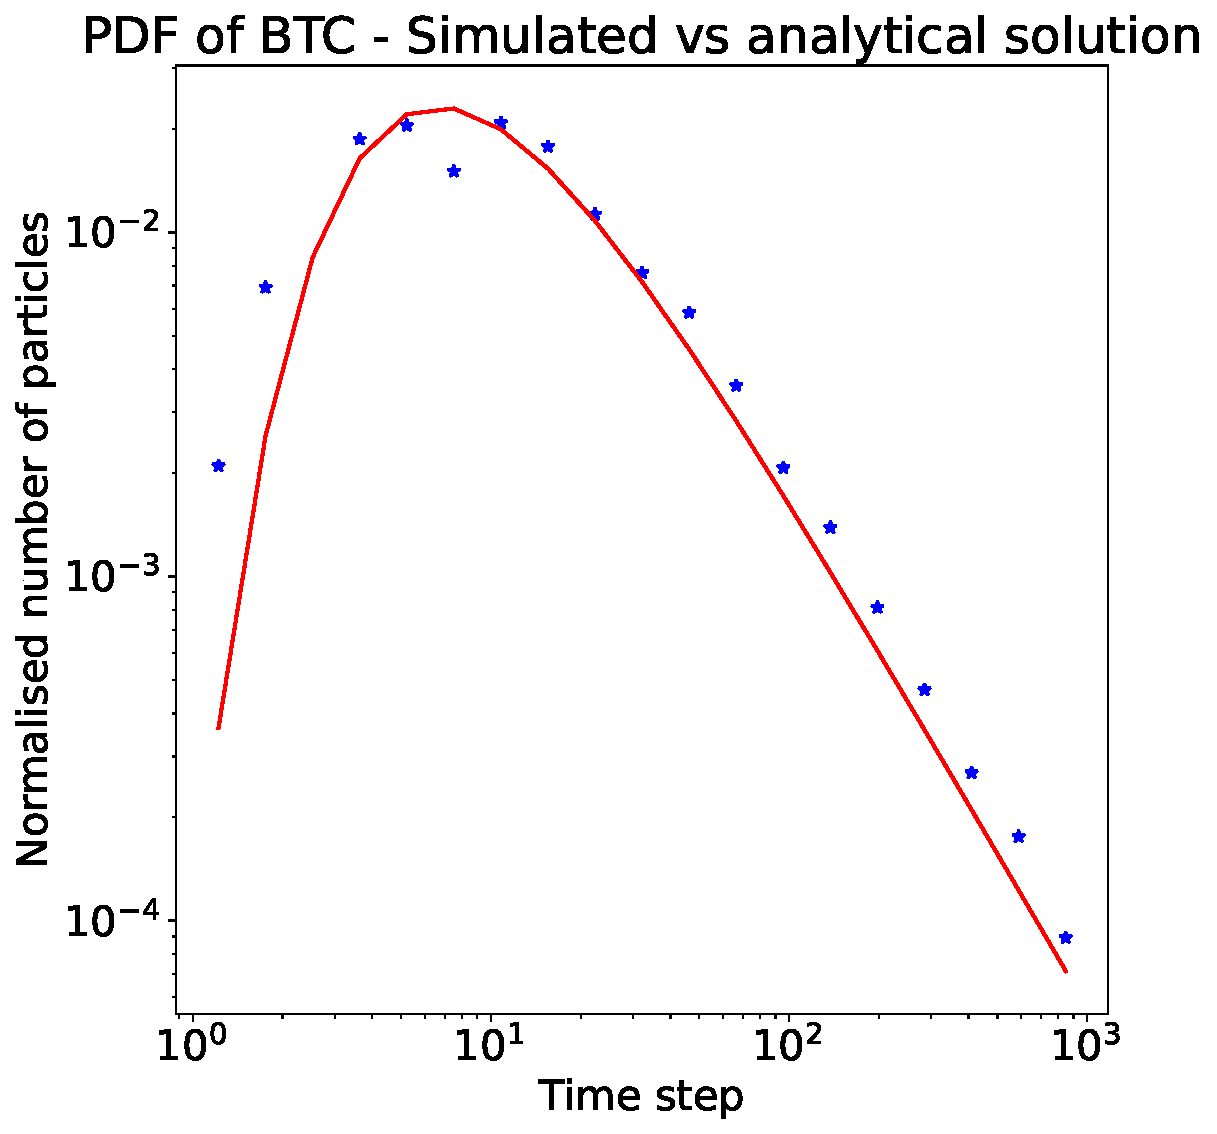
\includegraphics[width=\textwidth]{images/verificationSemi-infinite.pdf} % Replace with your image path
        \caption{Arrival times on the left absorbing boundary}
        \label{fig:subplotVerSemiInf}
    \end{subfigure}
    \caption{Verification of the code comparing two pdfs of the btc: blue dots represent the btc pdf from numerical simulation, solid red line is the analytical solution of the btc pdf for a semi-infinite domain}
    \label{fig:SemiInfinite}
\end{figure}

\end{document}